\section{Components of validation system}
\label{sec-webapplication}

The components of \textsf{Geant-val} web application and interactions between them are shown in the Fig.~\ref{fig:dataflow}.

\begin{figure}[h]
    \centering
    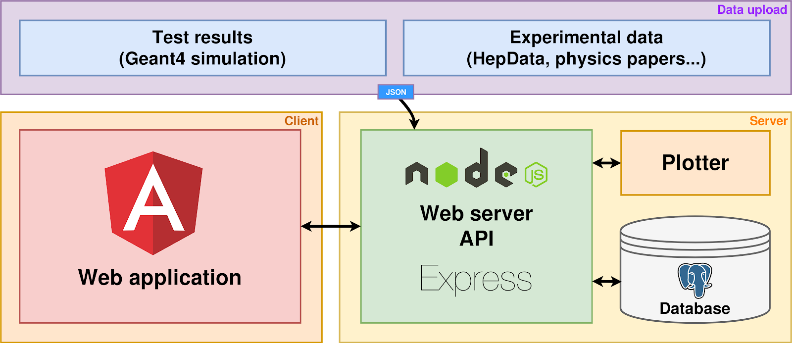
\includegraphics[width=0.8\textwidth,clip]{schema.png}
    \caption{Components of \textsf{Geant-val} web application and flow of data between them.}
    \label{fig:dataflow}
\end{figure}

\textbf{The server} is the core of the Geant4 validation system. It provides a web API that allows clients to access the database, respond to the clients' requests and generate high quality plots "on the fly" whenever they are requested using the ROOT~\cite{ROOT} data analysis framework.
It is written in JavaScript and runs with the Node.js engine~\cite{NodeJS}. 

\textbf{The database} is used for storing plots containing simulation results or experimental data, together with parameters describing these plots: tool name and version (e.g. \texttt{Geant4, 10.4.p02}), name of the test by which the plot was produced, or Inspire (HepData) ID of the article, etc. PostgreSQL~\cite{Postgre} is used as database management system for the application. The database instance is provided by the CERN Database-On-Demand service  % The database schema is designed in a way to allow scatter plots and histograms with unlimited number of optional test parameters in additional to a few mandatory ones to be stored.

% db schema

\textbf{A ROOT-based C++ plotting utility} was developed to produce high quality plots. It uses data in the JSON format which has been introduced as main interchange format between all parts of the application. The utility is not deeply integrated in the server infrastructure and can be used as a standalone application. It supports all types of application's data, can plot histograms with different binning on one canvas, and produce ratio plots. Ranges and scales of plot axes are selected automatically, with ability to override if necessary. % User-defined styles are also supported.

\textbf{Web interface} is user-friendly AngularJS~\cite{AngularJS} single page application which provides plots with tests results together with statistical analysis to the users.

%AngularJS is chosen because it allows to build efficient web applications with highly reusable components.

% The SPA contains 2 pages (see~\ref{sec-analyse} for details):
% \begin{itemize}
%     \item User layouts
%     \item Statistical comparisons
% \end{itemize}

%\begin{figure}[h]
%    \centering
%    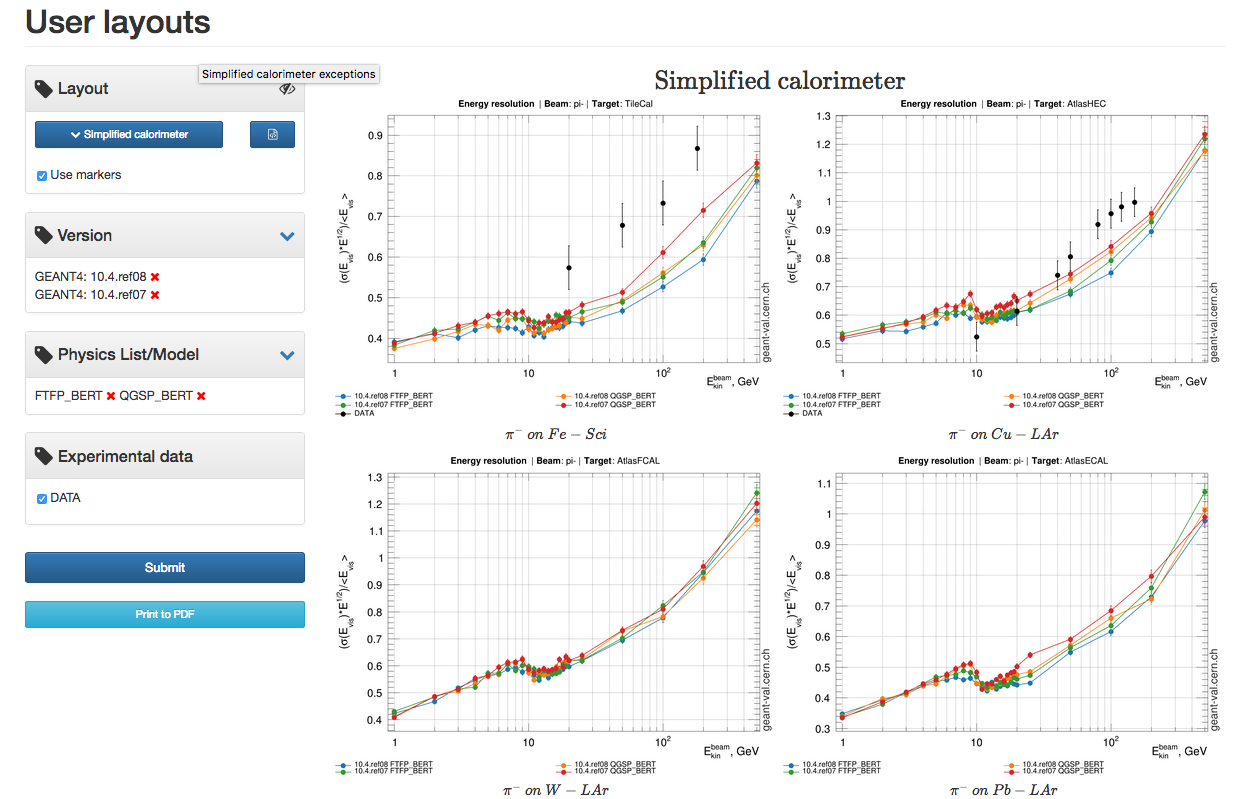
\includegraphics[width=0.8\textwidth,clip]{layout_sc.png}
%    \caption{Example of user defined layout for the Geant4 "simplified calorimeter" test showing test results for two Geant4 reference releases - 10.4.ref07 and 10.4.ref08.}
%    \label{fig:layouts}
%\end{figure}

%\textit{User layouts} page (see Fig.~\ref{fig:layouts}). Some Geant4 tests produce hundreds of different plots, but for fast "visual" validation it is often enough to compare only a small well-defined subset of them. The \textit{User layout} is an XML file describing what plots should be displayed and how should they be laid out on a page. User can use one of the existing layouts or define their own one (see Appendix~\ref{adx:XML-format}).
% is used to perform fast visual validation of Geant4.  
% One can use one of the existing templates or create and upload their own one. 
% It is possible to compare different versions between themselves or against experimental data. 
% If two or more Geant4 versions are selected, one can also select a "reference" dataset and plot the ratio of other datasets to it.

%\begin{figure}[h]
%    \centering
%    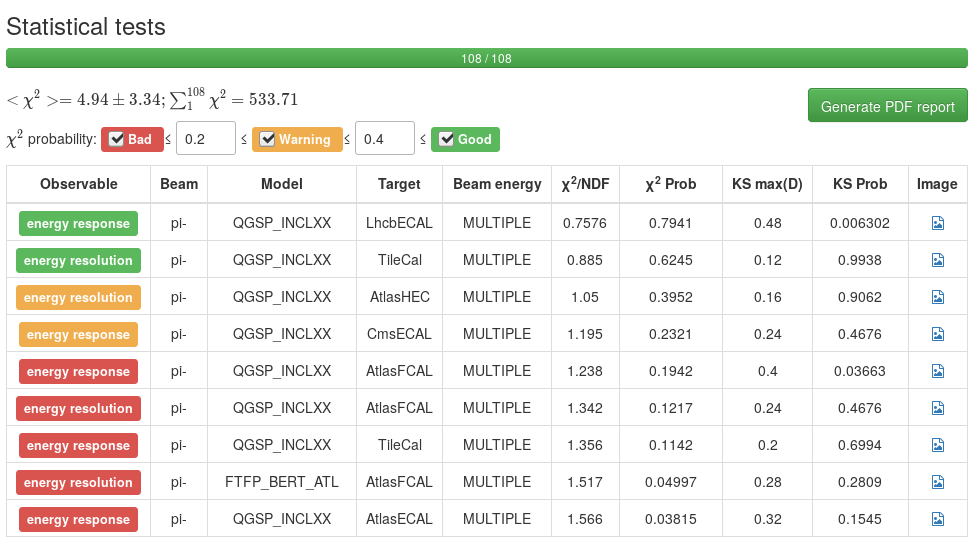
\includegraphics[width=0.8\textwidth,clip]{statcomparison.png}
%    \caption{Example of statistical comparison between two official Geant4 releases, 10.5.beta01 and 10.4.p02, for the "simplified calorimeter" test.}
%    \label{fig:statcomparison}
%\end{figure}

%\textit{Statistical comparisons} page (see Fig.~\ref{fig:statcomparison}) allows one to perform comparison of simulation with compatible experimental results using statistical tests. It displays results of statistical comparison for pairs of plots with the same parameters' values.
%Currently $\chi^2$ ($\chi^2/n.d.f.$, $\chi^2$ probability) and Kolmogorov-Smirnov (KS Max(D), KS probability) tests are implemented. All computations are performed asynchronously on the client side using JavaScript WebWorkers.
%For this purpose, JavaScript code to perform $\chi^2$ and Kolmogorov-Smirnov tests have been written, and their results cross-checked against the same statistical techniques implemented in the ROOT framework.


%On the \textit{experimental data} page (see Fig.~\ref{fig:exppage}) a summary table of available experimental data is displayed. The data is extracted from original articles or imported from HepDATA~\cite{hepdata} portal. % The experimental data is not linked with particular test and can be used by any tests if parameters match with simulation data.

%\begin{figure}[h]
%    \centering
%    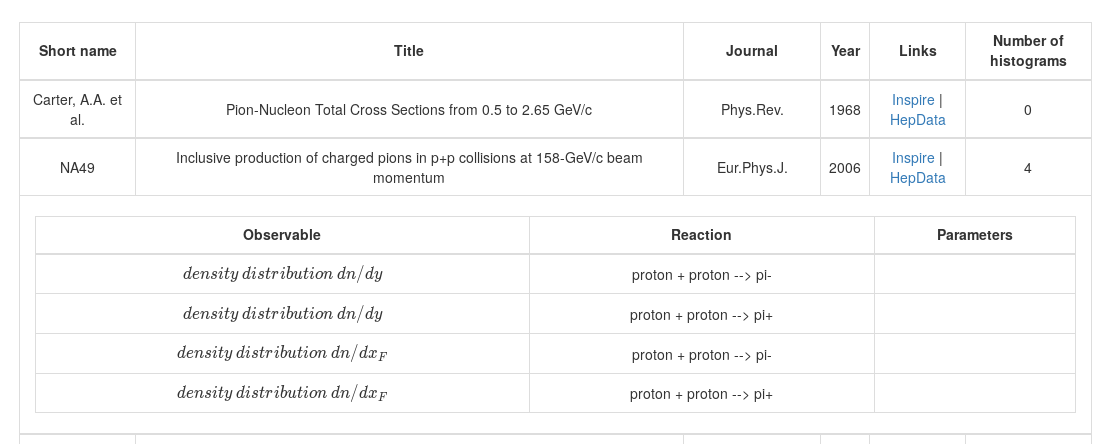
\includegraphics[width=0.8\textwidth,clip]{expdata.png}
%    \caption{Available experimental data.}
%    \label{fig:exppage}
%\end{figure}

Each plot on the website can be displayed as a static image produced by {\tt plotter} or as an interactive JSROOT~\cite{JSROOT} object, which allows changing axes ranges, scales and styles of the data "on the fly" in the same way as it can be done in ROOT. It is possible to export the plots in PNG, ROOT, EPS, Gnuplot~\cite{gnuplot} or \textsf{Geant-val} JSON format. 

Access to the test results produced with internal Geant4 releases is restricted to the Geant4 developers authenticated via CERN Single Sign-On. For public Geant4 releases the access is open to anyone.

%Don't forget to give each section, subsection, subsubsection, and
%paragraph a unique label (see Sect.~\ref{sec-1}).

%For one-column wide figures use syntax of figure~\ref{fig-1}
%\begin{figure}[h]
% Use the relevant command for your figure-insertion program
% to insert the figure file.
%\centering
%\includegraphics[width=1cm,clip]{tiger}
%\caption{Please write your figure caption here}
%\label{fig-1}       % Give a unique label
%\end{figure}

%For two-column wide figures use syntax of figure~\ref{fig-2}
%\begin{figure*}
%\centering
% Use the relevant command for your figure-insertion program
% to insert the figure file. See example above.
% If not, use
%\vspace*{5cm}       % Give the correct figure height in cm
%\caption{Please write your figure caption here}
%\label{fig-2}       % Give a unique label
%\end{figure*}

%For figure with sidecaption legend use syntax of figure
%\begin{figure}
% Use the relevant command for your figure-insertion program
% to insert the figure file.
%\centering
%\sidecaption
%\includegraphics[width=5cm,clip]{tiger}
%\caption{Please write your figure caption here}
%\label{fig-3}       % Give a unique label
%\end{figure}

%For tables use syntax in table~\ref{tab-1}.
%\begin{table}
%\centering
%\caption{Please write your table caption here}
%\label{tab-1}       % Give a unique label
% For LaTeX tables you can use
%\begin{tabular}{lll}
%\hline
%first & second & third  \\\hline
%number & number & number \\
%number & number & number \\\hline
%\end{tabular}
% Or use
%\vspace*{5cm}  % with the correct table height
%\end{table}

To manage a set of Geant4 tests and their configurations, a {\tt mc-config-generator} \textbf{Python-based framework} was developed. It allows one to configure and run test jobs in various batch systems (CERN LSF, HTCondor, Torque PBS), and to convert the results into  JSON format for further uploading to the application database. The framework is not Geant4-specific, and can be used with other projects (e.g., Pythia8). Source code is available in corresponding Git repository\footnote{https://gitlab.cern.ch/GeantValidation/geant-config-generator}.

